\chapter{Differential equations} 
The theory in this chapter is based on \cite{diffandcomplex}. In this chapter linear differential equations of the first order, separable differential equations, and their solutions will be described with corresponding examples. In this report, the Leibniz notation is used for derivatives. 
\\
\\
Before describing an RC circuit mathematically, the concept of differential equations has to be described. Differential equations are important tools to describe dynamic physical systems. An example of this could be an equation to describe an increasing population. The growth of a population is usually a function of that same population.
\begin{definition}{Differential equation}{}
A differential equation is an equation, which contains a function, and one or more of its derivatives.
\end{definition}
\noindent%Phenomena
These equations have a function as a solution, rather than a number. 
\\
A differential equation would look something like this: $\frac{dy}{dx} = y$. This equation asks: "What function is its own derivative?", which is of course $y=e^x+C$.
\\
\setlength\intextsep{0pt}
\begin{wrapfigure}{r}{7cm}[H]
	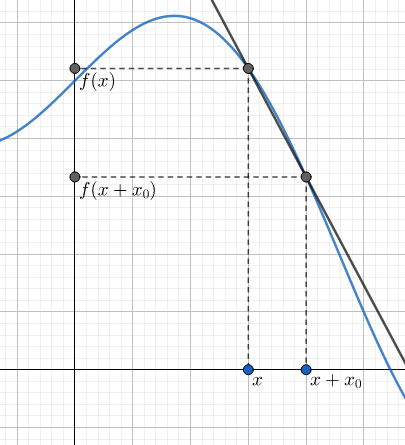
\includegraphics[scale=0.5]{fig/img/dydx.png}
	\caption{A function $f$, shown with a secant from $x$ to $x+x_0$}\label{wrap-fig:1}
\end{wrapfigure}
In this context $dy$ and $dx$ can be perceived as small changes in $y$, and small changes in $x$. The slight change in $y$, with respect to $x$, can then be described as $\dfrac{dy}{dx}$.
\\
This can be expressed formally as:
\\
\begin{align*}
	\dfrac{dy}{dx} =& y'(x) \\
	\dfrac{dy}{dx} =& \lim_{x_0\to 0} \dfrac{y(x+x_0)-y(x)}{x_0}
\end{align*}
A differential equation can either have a general solution or a particular solution. When finding the general solution, there is no initial condition to determine the constant $C$. Finding a particular solution requires an initial condition, from which the constant $C$ can be found.

\clearpage

\begin{definition}{Order of a differential equation}{}
The order of a differential equation is determined by the highest order of derivative present in the equation.
\end{definition} 

\noindent
\textbf{Examples of differential equations of different orders:}
\\
A first order differential equation:
$$y=4\frac{dy}{dx} $$
A second order differential equation:
$$\frac{d^2y}{dx^2}+\frac{dy}{dx}+y = 5\frac{dy}{dx}$$
And a third order differential equation:
$$\frac{d^3y}{dx^3} - 9\frac{d^2y}{dx^2} + 15\frac{dy}{dx} + 25y = 0$$

\section{Linear differential equations}
There are two types of differential equations, linear and non-linear. A linear differential equation is a linear polynomial that consists of a function and its derivatives.
\begin{definition}{$N$'th order linear differential equation}{}
A linear $N$'th order differential equation is an equation, which can be written in the following way:
\begin{align*}
\sum_{k=0}^{N}\left(\dfrac{d^ky}{dx^k}a_k(x)\right)+b(x)=0,
\end{align*}
where $a_k(x)$ are continuous functions on a given interval.
\end{definition}
\subsection{Solving a linear differential equation of the first order}
=======
Solving  a differential equation is not always easy or possible. For differential equations in certain forms, a general solution can be form.

\begin{theorem}{General solution to a linear differential equation of the first order}{linethe}
A first order linear differential equation in the form of
<<<<<<< HEAD
>>>>>>> master
=======
>>>>>>> master
\begin{align} \label{FODE_form}
\dfrac{dy}{dx}+h(x)y=g(x),
\end{align}
has the general solution
\begin{align} \label{FODE_solution}
y=e^{-H(x)}\left(\int e^{H(x)}g(x)\ dx+C\right),
\end{align}
where $H(x)$ is the antiderivative of $h(x)$, $h$ and $g$ are continuous in a given interval, and $C\in \mathbb{R}$.
\end{theorem}

\begin{prof}{}{}
\Cref{FODE_form} is multiplied by $e^{H(x)}$ on each side:
\begin{align*}
\left(\dfrac{dy}{dx}+h(x)y\right)e^{H(x)}=&g(x)e^{H(x)}
\\
\dfrac{dy}{dx}e^{H(x)}+h(x)ye^{H(x)}=&g(x)e^{H(x)}
\end{align*}
Considering the chain rule, and product rule, the left-hand side of the equation can be rewritten as:
\begin{align*}
\dfrac{d}{dx}\left(e^{H(x)}y\right)=g(x)e^{H(x)}
\end{align*}
This is because the left-hand side, when differentiated, becomes:
\begin{align*}
\dfrac{d}{dx}\left(e^{H(x)}y\right)=&\dfrac{d}{dx}\left(e^{H(x)}\right)y+\dfrac{dy}{dx}e^{H(x)} \\
 =& h(x)ye^{H(x)}+\dfrac{dy}{dx}e^{H(x)}
\end{align*}
Both sides are then integrated with respect to $x$:
\begin{align*}
\int\dfrac{d}{dx}\left(e^{H(x)}y\right)\ dx=&\int g(x)e^{H(x)}\ dx
\\
e^{H(x)}y=&\int g(x)e^{H(x)}\ dx+C,
\end{align*}
where $C$ is the constant of integration from the left side of the  equation. By multiplying both sides with $e^{-H(x)}$, the general solution can be found.
\begin{align}
y=e^{-H(x)}\left(\int g(x)e^{H(x)}\ dx+C\right)
\end{align}
\end{prof}

\begin{example}{Solving a linear differential equation of first order}{}
Consider the following differential equation with the given initial condition.
\begin{align}
	\dfrac{dy}{dx}-2y=e^x  \label{ODE_ex}\\ 
	y(0) =& 5 \nonumber
\end{align}
From \eqref{ODE_ex}, it is seen that it can be identified in the form of \eqref{FODE_form}, where:
%This equation can be rearranged to fit the form of \eqref{FODE_form}, and a general solution, to the differential equation, can then be found using \eqref{FODE_solution}:
\begin{align*}
	h(x) =& -2 \\
	g(x) =& e^x \\
	H(x) =& \int{-2 dx} \\
	     =& -2x + C
\end{align*}
Substituting the functions in \eqref{FODE_solution} with $H(x)$ and $g(x)$, we get: 
\begin{align*}
	y(x)=&e^{2x+C}(\int{e^{-2x-C}e^x\ dx}+C) \\
	y(x)=&e^{2x}e^{C}(e^{-C}\int{e^{-2x}e^{x}\ dx}+C) \\
	y(x)=&e^{2x}(\int{e^{-x}\ dx}+C_{1})
\end{align*}
Where $C_{1}$ is the new constant of integration, $C_1=e^{C}C$. \\
The integral of $e^{-x}$ can then be found. The following result is then reduced:
\begin{align*}
	y(x)=&e^{2x}(-e^{-x}+C_{2}+C_{1}) \\
	y(x)=&-e^x+C_{3} \cdot e^{2x}
\end{align*}
Where $C_{3}$ is the new constant of integration, $C_{3}=C_{2}+C_{1}$. $C_{3}$ is then calculated from the initial condition:
\begin{align*}
	y(0)=&5 \\
	5=&-e^0+C_{3} \cdot e^{2 \cdot 0} \\
	5 =& C_{3}-1 \\
	C_{3} =& 6
\end{align*}
The particular solution to the differential equation is then:
\begin{align*}
	y(x) = -e^x+6e^{2x}
\end{align*}
To check the validity of this solution, it is substituted into the differential equation:
\begin{align*}
	e^x =& \dfrac{dy}{dx} -2y \\
	e^x =& -e^x+12e^{2x} -2(-e^x+6e^{2x})  \\
	e^x =& -e^x+2e^x  \\
	e^x =& e^x
\end{align*}
This must then be a particular solution to the given differential equation.
\end{example}

\section{Separable differential equations}\label{SepDiff}
\begin{definition}{Separable differential equations}{def:SDE}
Given a differential equation in the following form. 
$$\frac{dy}{dx} = f(x,y)$$
The equation is said to be separable if the right-hand side of the equation can be expressed as a function $g(x)$ that depends only on $x$, times a function $p(y)$ that depends only on $y$:
\begin{align}
f(x,y)=g(x)p(y)
\end{align}
Where $g(x)$ and $p(y)$ are continuous in a given interval.
\end{definition}
\noindent
By definition \ref{def:SDE} a first order, separable differential equation can be written as:
\begin{align}
	\frac{dy}{dx}=g(x)p(y)
\end{align}
The equation can then be rewritten and solved as follows:
\begin{align}
	h(y)dy=g(x)dx,
\end{align}
where $h(y) = \frac{1}{p(y)}$. Both sides of the equation are then integrated:
 \begin{align}
 	\int h(y)dy =&\int g(x)dx   \\
 	H(y)=&G(x)+C \label{SDEG}
 \end{align}
 
The two constants are merged into one constant $C$. This is the general solution to a differential equation. \cite{diffandcomplex}

\subsection{Justification} 
To show that the differentials $dy$ and $dx$ in $\frac{dy}{dx}$ can be treated algebraically when solving \eqref{2_4}:
 \begin{align}
	\frac{dy}{dx} &= g(x)p(y)\nonumber\\
	h(y)\frac{dy}{dx} &= g(x)\label{eq:1}
 \end{align}
Then by letting $H(y)$ be the antiderivative of $h(y)$, and $G(x)$ be the antiderivative of $g(x)$, equation \eqref{eq:1} can be rewritten as: 
 \begin{align}
 	\frac{dH}{dy}\frac{dy}{dx} &= \frac{dG}{dx}\label{eq:2}
 \end{align}
Using the chain rule for differentiation, $\frac{dH}{dy}\frac{dy}{dx}$ can be written as the derivative of the composite function $H(y(x))$:
 \begin{align*}
	\frac{d}{dx} H(y(x)) &= \frac{dH}{dy}\frac{dy}{dx}.
 \end{align*}
In \ref{eq:2} this term can be substituted:
 \begin{align}
 	\frac{d}{dx}H(y(x)) &= \frac{dG}{dx}\label{eq:3}.
 \end{align}
Equation \ref{eq:3} shows that $H(y(x))$ and $G(x)$ have the same derivative, and must differ by a constant after integrating both sides:
 \begin{align*}
 	H(y(x)) &= G(x) + C
 \end{align*}
This shows that the same result is found whether $\frac{dy}{dx}$ is split algebraically, or the antiderivatives are used together with the chain rule for differentiation. Therefore, it is justified to treat $\frac{dy}{dx}$ algebraically.


\begin{example}{Solving a separable differential equation}{}
Given the differential equation and initial condition:
\begin{align*}
	\dfrac{dy}{dx} =& y^2 4x \\
	y(1) =& \dfrac{1}{3},
\end{align*}
what would the particular solution be?
\\ \\
The terms, in this case, are simple to separate: 
\begin{align*}
	\dfrac{dy}{dx} y^{-2} =& 4x \\
	y^{-2} dy =& 4x dx 
\end{align*}
Both sides of the equation are then integrated, and solved for $y$:
\begin{align*}
	\int{y^{-2} dy} =& \int{4x dx} \\
	-y^{-1} =& 2x^2 +C \\
	y =& \dfrac{1}{-2x^2-C}
\end{align*}
The integration constant can then be found, using the initial condition:
\begin{align*}
	y(1) =& \dfrac{1}{3} \\
	\dfrac{1}{3} =& \dfrac{1}{-2 \cdot 1^2-C} \\
	3 =& -2-C \\
	C =& -5
\end{align*}
The particular solution to this equation is then:
\begin{align*}
	y(x) = \dfrac{1}{-2x^2+5}
\end{align*}

The validity of the solution can be checked, by substituting the solution in the equation:
\begin{align*}
	\dfrac{dy}{dx} =& y^24x \\
	y(1) =& \dfrac{1}{3}  \\
	\\
	\dfrac{d}{dx} \left(\dfrac{1}{-2x^2+5}\right) =& \dfrac{4x}{(-2x^2+5)^2} \\
	-4x\left(\dfrac{-1}{(-2x^2+5)^2}\right)  =& \dfrac{4x}{(-2x^2+5)^2} \\
	\dfrac{4x}{(-2x^2+5)^2} =& \dfrac{4x}{(-2x^2+5)^2}
\end{align*}
A particular solution to the equation has then been found.
\end{example}
